\documentclass[a4paper,11pt]{article}
\usepackage{amsmath}
\usepackage{hyperref}
\usepackage{graphicx}
\usepackage{listings}
\usepackage{color}

\definecolor{gray}{rgb}{0.5,0.5,0.5}
\newcommand{\convolution}{\ensuremath{+\negmedspace\negmedspace\negmedspace\times}}

%% Provide \Autoref; the \autoref with a printed capital
\def\figureautorefname{figure}
\def\tableautorefname{table}
\def\partautorefname{part}
\def\appendixautorefname{appendix}
\def\equationautorefname{equation}
\def\AMSautorefname{equation}
\def\theoremautorefname{theorem}
\def\enumerationautorefname{case}
\def\Autoref#1{%
  \begingroup
  \edef\reserved@a{\cpttrimspaces{#1}}%
  \ifcsndefTF{r@#1}{%
    \xaftercsname{\expandafter\testreftype\@fourthoffive}
      {r@\reserved@a}.\\{#1}%
  }{%
    \ref{#1}%
  }%
  \endgroup
}
\def\testreftype#1.#2\\#3{%
  \ifcsndefTF{#1autorefname}{%
    \def\reserved@a##1##2\@nil{%
      \uppercase{\def\ref@name{##1}}%
      \csn@edef{#1autorefname}{\ref@name##2}%
      \autoref{#3}%
    }%
    \reserved@a#1\@nil
  }{%
    \autoref{#3}%
  }%
}

 
\author{Maarten Inja \and Patrick de Kok}
\title{MLPR: Lab 1}

\lstset{
  language=Octave,
  basicstyle=\footnotesize,
  numbers=left,
  numberstyle=\tiny\color{gray},
  stepnumber=5,
  showspaces=false,
  showstringspaces=true
  showtabs=false,
  frame=single,
  title=\lstname,
  breaklines=true,
}
\begin{document}
\maketitle

\section*{Exercise 1}
\begin{figure}[h]
  \caption{A plot of the dataset.  The red ``$\color{red}+$'' and magenta ``$\color{magenta}\circ$'' represent the training and test data points of class A.  The blue ``$\color{blue}\times$'' and black ``$\convolution$'' represent the training and test data points of class B.}
  \label{plot1}
  \begin{center}
    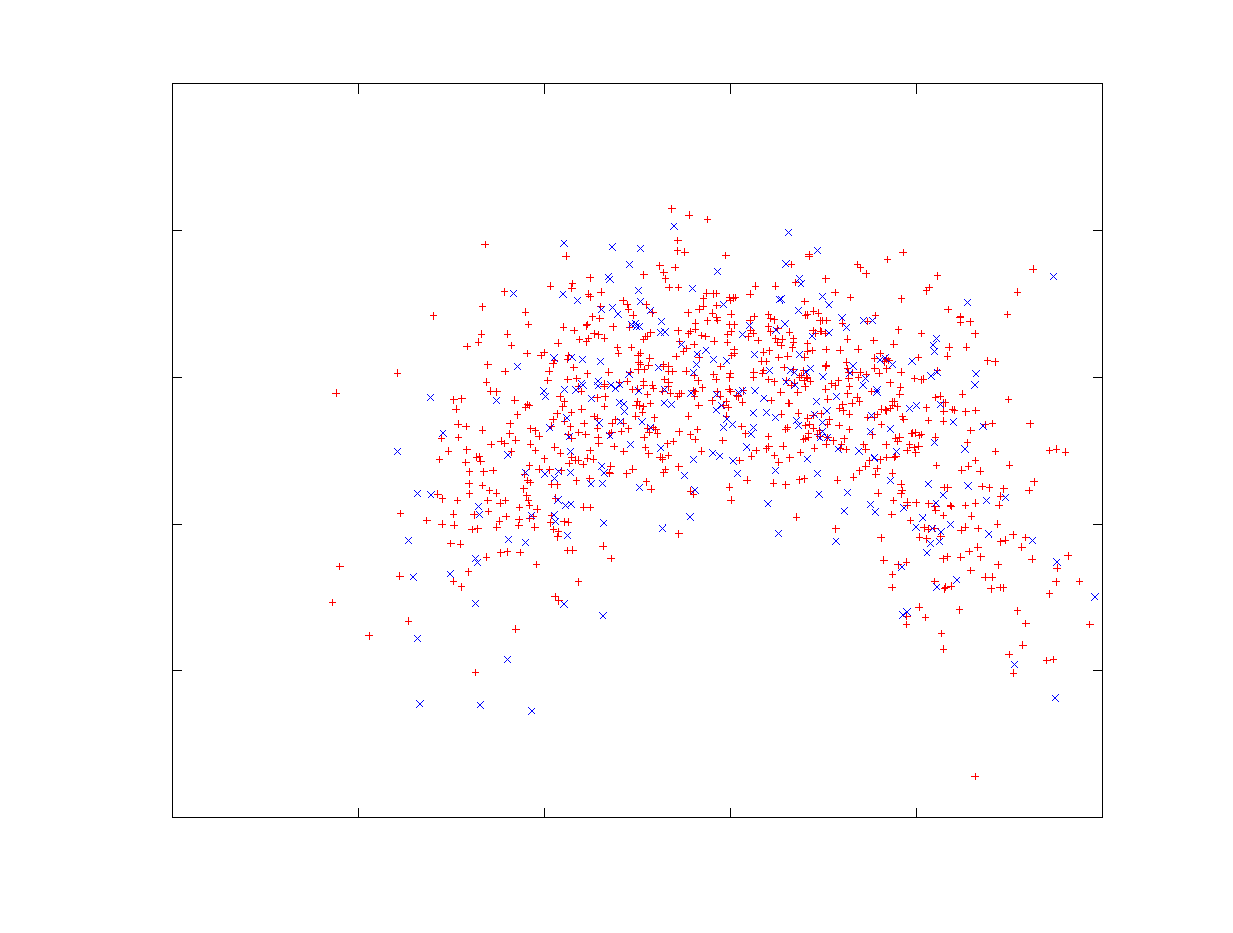
\includegraphics[width=0.6\paperwidth]{plot1}
  \end{center}
\end{figure}

Our training and test data sets are generated through the Matlab code presented in \autoref{code}.  A graphical representation is given in \autoref{plot1}.

\lstinputlisting[caption={The code which generates our data set},label=code]{preprocess_data.m}

\section*{Exercise 2}
\begin{enumerate}
\item \textit{Train a $k$NN classifier, with $k$ = 1, on the training data, evaluate its performance on the test data and
compute the test error.}
\item \textit{Try other values for $k$ ($k$ = 1, 3, $\ldots$), plot how the test error evolves as a function of k and include the
resulting graph in your report. Which value of k would you use, and why? Can you derive any definite
conclusions from this experiment?
}

% We gebruiken alleen maar oneven waarden voor $k$; je kunt anders een gelijke stemming hebben bij welke klasse een test sample hoort.

\end{enumerate}

\label{sec:two}
Confusion matrices of the $k$NN with $1 \leq k \leq 20$:

\begin{table}
  \caption{TA = True A; TB = True B; CA = classified as A; CB = classified as B.}
\begin{tabular}{lcrr}
$k$ && CA & CB \\ \\
 1 & TA & 199 &    51 \\
& TB &  34 &   216 \\
 2 & TA & 205 &    45 \\
& TB &  34 &   216 \\
 3 & TA & 212 &    38 \\
& TB &  33 &   217 \\
 4 & TA & 217 &    33 \\
& TB &  35 &   215 \\
 5 & TA & 214 &    36 \\
& TB &  30 &   220 \\
 6 & TA & 217 &    33 \\
& TB &  31 &   219 \\
 7 & TA & 216 &    34 \\
& TB &  31 &   219 \\
 8 & TA & 221 &    29 \\
& TB &  32 &   218 \\
 9 & TA & 216 &    34 \\
& TB &  30 &   220 \\
 10 & TA & 217 &    33 \\
& TB &  32 &   218 \\
 11 & TA & 214 &    36 \\
& TB &  29 &   221 \\
 12 & TA & 215 &    35 \\
& TB &  28 &   222 \\
 13 & TA & 215 &    35 \\
& TB &  31 &   219 \\
 14 & TA & 216 &    34 \\
& TB &  31 &   219 \\
 15 & TA & 216 &    34 \\
& TB &  31 &   219 \\
 16 & TA & 213 &    37 \\
& TB &  31 &   219 \\
 17 & TA & 215 &    35 \\
& TB &  35 &   215 \\
 18 & TA & 215 &    35 \\
& TB &  34 &   216 \\
 19 & TA & 215 &    35 \\
& TB &  36 &   214 \\
 20 & TA & 216 &    34 \\
& TB &  33 &   217 \\
\end{tabular}
\end{table}

\section*{Exercise 3}
\begin{enumerate}
    \item \textit{Discuss briefly (200 words) what the advantage would be of using a method like cross-validation or
bootstrapping in this context.}

% Je kunt ook \autoref gebruiken. Zit standaard in hyperref. Ik heb ook een definitie voor \Autoref toegevoegd; dat is \autoref, maar begint dan met een hoofdletter :)
The method used in section \ref{sec:two} biases the machine towards the test set. The test set should normally be
used to evaluate the machine learning algorithm and/or its parameters. The test set should not be used to 
select a model, as was implied in section \ref{sec:two}. 
Cross-validation can be used to fairly evaluate models using solely the training set without the risk of 
introducing a bias for one specific validation set. 

Bootstrapping 

\item \textit{Implement 10-fold cross-validation, and give an estimate for a good value of $k$.}

\item \textit{Can you use this estimate of $k$ in your final classifier? What is the use of doing cross-validation?}

\item \textit{ How do you compute the test error? What is it an estimate of? What would be the use of a validation
set? }



\end{enumerate}

\end{document}
